\section{Les diagrammes de séquences}
 
Les diagrammes ci-dessous décrivent les séquences d’extraction des données à partir des stations météo sencrop et davis vantage pro 2 ansi que leurs chargment dans des bases de données intermédiaire.

\subsection{Séquence pour la station sencrop.}
Sencrop met à disposition de ses clients, détenteurs d’une de leurs stations, une plateforme de visualisation des relevés. Cette plateforme présente des données en générale de façons agrégés mais permettant d’avoir une bonne lecture de la situation météorologique selon une plage de temps que l’on souhaite. Elle met également à disposition une API, qui par des requêtes bien précises, permet d’avoir les relevés brutes.  

Il faut donc a avoir un compte sencrop et se connecter à l’ \gls{API}. une fois la connexion établit, un jeton ayant une date d’expiration est généré, et l’on peut faire ainsi une requête. Ce processus peut donc être automatiser via un script python et être exécuté régulièrement via un gestionnaire de tâches. La grande difficulté réside dans le fait de bien comprendre en amont, la structure des requête c’est-à-dire le nombre et le type de paramètres qu’il faut envoyer mais aussi la structure des données que l’on reçoit. C’est pour cela que sencrop a prévu une documentation pour pouvoir utiliser l’API. 
\newline
\url{https://developer.sencrop.com/guide/}  
\begin{figure}[!h]
    \label{diagramme de séquence stéation sencrop}
    \centering
     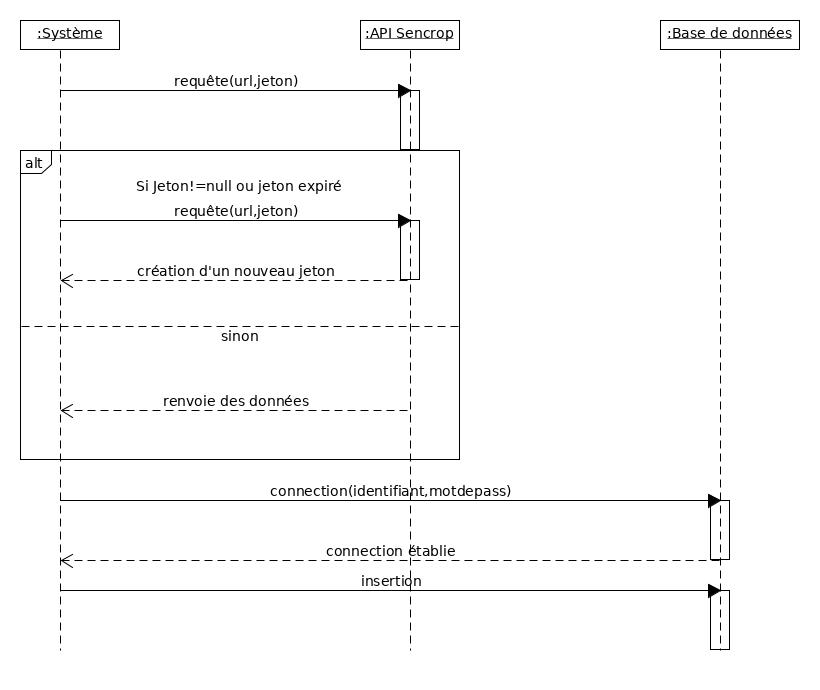
\includegraphics[width=.7\textwidth]{images/sencrop_senquence_diagrame.jpg}
    \caption{diagramme de séquence pour l'extraction et le chargement des données de la station sencrop}
  
\end{figure}

\subsection{Séquence pour la station davis vantage pro 2} 
La station météo davis vantage pro 2 génère des fichiers au format .wlk. Ces fichiers sont modifiés quotidiennement et ne contienent que les données du mois courant. Ainsi par exemple pour le mois d’août 2018 un fichier de nom 2018\_08.wlk sera généré. Celui-ci sera modifié quotidiennement pour contenir tous le données à partir du 01 jusqu’au jour précédent. Un logiciel, fourni par l’entreprise propriétaire, pour décoder les fichiers .wlk existe mais il n’est pas gratuit.Plus encore, il n’est pas pas multiplateforme et l’utilisation de celui-ci en ligne de commande pour automatiser les tâches est quasi-impossible car il nécessité plusieurs paramétrés. Nous nous sommes donc tournés vers des outils libres qui existeraient sur internet pour décoder les fichiers wlk.J'ai ainsi trouvé un utilitaire permettaant non seulement de décoder les fichiers .wlk mais aussi de générer des fichiers au format sql pour alimenter une base de données. Ceci nous a beaucoup aidé car il ne restait plus que la tâche d'automatisation  de décodage des fichiers .wlk et celui de l’insertion. Mais il s’est avéré qu' à certains endroits, l’utilitaire produsait des erreurs de sorti. La grande difficulté fut de pouvoir personnalisé les sortis attendues pour qu’elles correspondent aux résultats escomptés. 

\begin{figure}
    
    \centering
     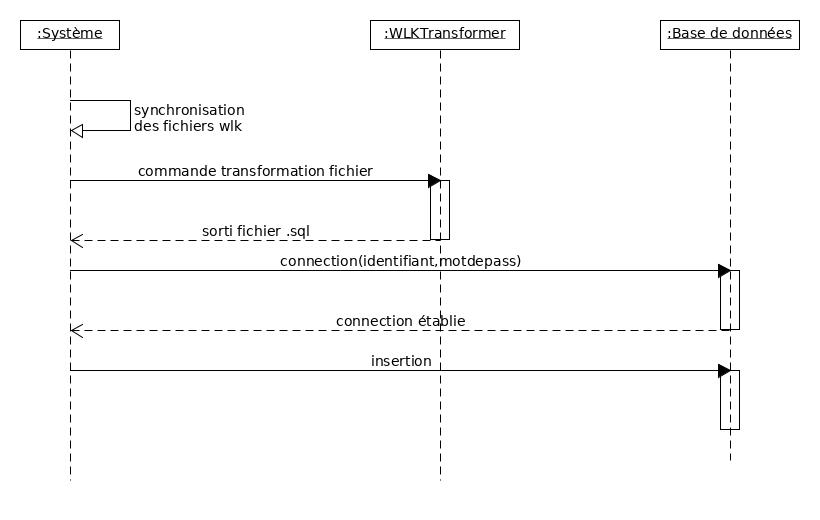
\includegraphics[width=.7\textwidth]{images/davis_senquence_diagrame.jpg}
     \caption{ Séquence pour l'extraction et le chargement des données de la station Davis vantage pro2}
     \label{diagramme de séquence station sencrop}
\end{figure}


\begin{figure}[!h]
    \centering
     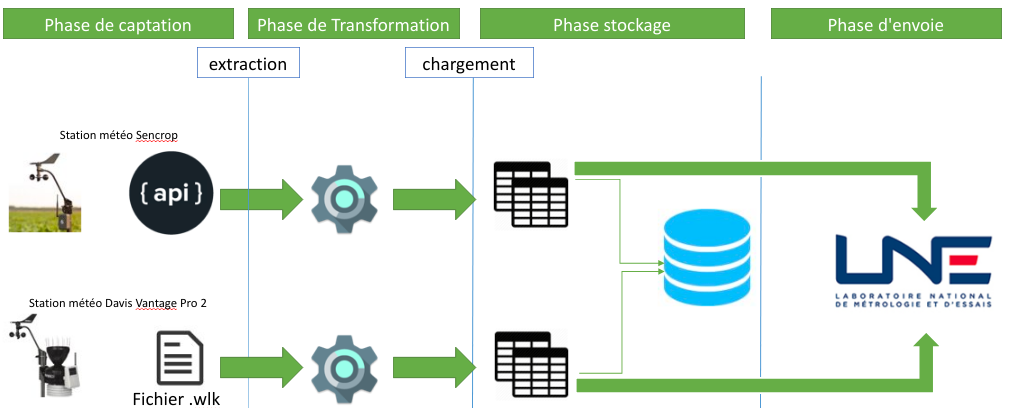
\includegraphics[width=1\textwidth]{images/processusOperose.png}
     \caption{ Séquence d'extraction de chargement et d'envoie données pour le projet OPEROSE}
     \label{diagremme de séquence station Davis}
\end{figure}

\section{Le diagramme de paquetage}
Le programme d'extraction et de chargement des données météo des deux stations a été implémenté de façon modulaire dans lequel chaque module est indépendants. Nous avons donc un paquet \textbf{SencropDataExport} dans lequel se trouvent :
\begin{itemize}
    \item une classe pour la connection et les requêtes vers l'API sencrop
    \item une classe pour la connection et les requêtes vers la base de données
    \item des classes pour l'extraction et le chargement des données(par jour, par heure et par 15minutes d'intervalles) dans une base de données intermédiaire.
    \item une classe qui migre les données de la base intermédiaire à la base de données générique
    \item une classe qui génère les fichiers qui devront être envoyés au LNE.
\end{itemize}
et un paquet \textbf{DavisDataExport} dans lequel se trouvent : 
\begin{itemize}
    \item une classe de connection à la base de données
    \item une classe qui décode les fichiers .wlk  et exporte les données dans une base de données intermédiaire
    \item une classe qui migre les onnées dans de la base intermédiare à la base de données générique
    \item une classe qui génère les fichiers qui devront être envoyés au LNE.
\end{itemize}

\begin{figure}[!h]
    \centering
    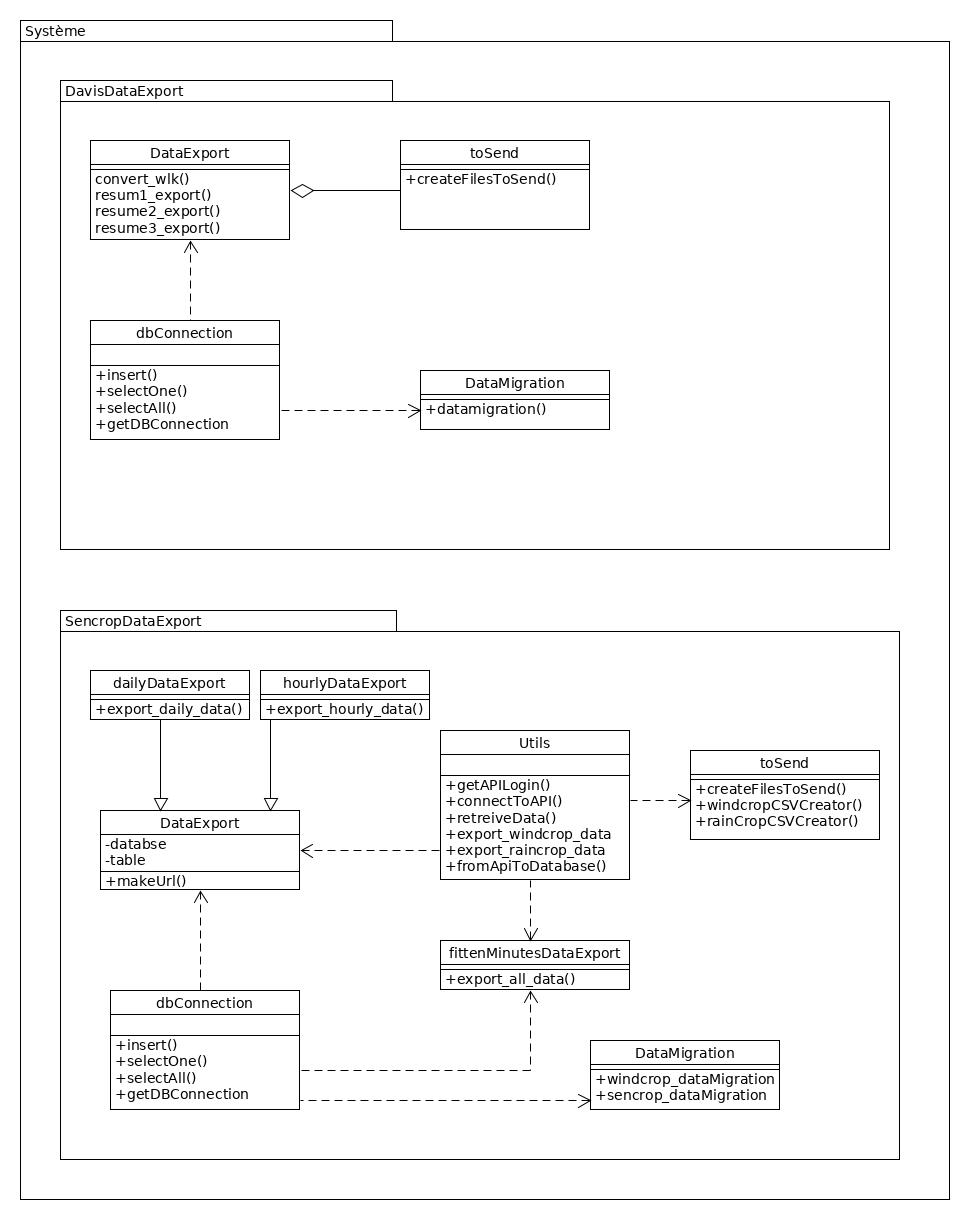
\includegraphics[height=.8\textheight]{images/package_diagramme.jpg}
    \caption{Diagramme des paquetages}
    \label{fig:Diagramme des paquetages}
\end{figure}
     

